% vim: set textwidth=78 autoindent:

% when the revision of a section has been finalized,
% comment out the following line:
%\updatedisclaimer

\section{Coordinate Reference Systems}\label{sec:crs}
\begin{tabular}{p{3.5cm}p{6cm}p{6cm}}
\multirow{2}{*}{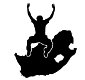
\includegraphics[width=2.5cm]{logo}} & Objectives: &
Understanding of Coordinate Reference Systems. \\
& & \\
& Keywords: & 
Coordinate Reference System (CRS), Map Projection, On the Fly Projection,
Latitude, Longitude, Northing, Easting  \\
\hline
\end{tabular}

\subsection{Overview}\label{subsec:overview}

\textbf{Map projections} try to portray the surface of the earth or a portion of the
earth on a flat piece of paper or computer screen. A \textbf{coordinate reference
system} (CRS) then defines, with the help of coordinates, how the
two-dimensional, projected map in your GIS is related to real places on the
earth. The decision as to which map projection and coordinate reference
system to use, depends on the regional extent of the area you want to work
in, on the analysis you want to do and often on the availability of data.

\subsection{Map Projection in detail}

A traditional method of representing the earth's shape is the use of globes.
There is, however, a problem with this approach. Although globes preserve the
majority of the earth's shape and illustrate the spatial configuration of
continent-sized features, they are very difficult to carry in one's pocket.
They are also only convenient to use at extremely small scales (e.g. 1 : 100
million).

Most of the thematic map data commonly used in GIS applications are of
considerably larger scale. Typical GIS datasets have scales of 1:250 000 or
greater, depending on the level of detail. A globe of this size would be
difficult and expensive to produce and even more difficult to carry around.
As a result, cartographers have developed a set of techniques called
\textbf{map projections} designed to show, with reasonable accuracy, the
spherical earth in two-dimensions.

When viewed at close range the earth appears to be relatively flat. However
when viewed from space, we can see that the earth is relatively spherical.
Maps, as we will see in the upcoming map production topic, are
representations of reality. They are designed to not only represent features,
but also their shape and spatial arrangement. Each map projection has
\textbf{advantages} and \textbf{disadvantages}. The best projection for a map
depends on the
scale of the map, and on the purposes for which it will be used. For example,
a projection may have unacceptable distortions if used to map the entire
African continent, but may be an excellent choice for a \textbf{large-scale
(detailed) map} of your country. The properties of a map projection may also
influence some of the design features of the map. Some projections are good
for small areas, some are good for mapping areas with a large East-West
extent, and some are better for mapping areas with a large North-South
extent. 

\subsection{The three families of map projections}

The process of creating map projections can be visualised by positioning a
light source inside a transparent globe on which opaque earth features are
placed. Then project the feature outlines onto a two-dimensional flat piece
of paper. Different ways of projecting can be produced by surrounding the
globe in a \textbf{cylindrical} fashion, as a \textbf{cone}, or even as a
\textbf{flat surface}. Each of
these methods produces what is called a map \textbf{projection family}.
Therefore, there is a family of \textbf{planar projections}, a family of
\textbf{cylindrical projections}, and another called \textbf{conical
projections} (see Figure \ref{fig:projfamilies})  

\begin{figure}[ht]
   \begin{center}
   \caption{The three families of map projections. They can be represented by
a) cylindrical projections, b) conical projections or c) planar projections.}
\label{fig:projfamilies}\smallskip
   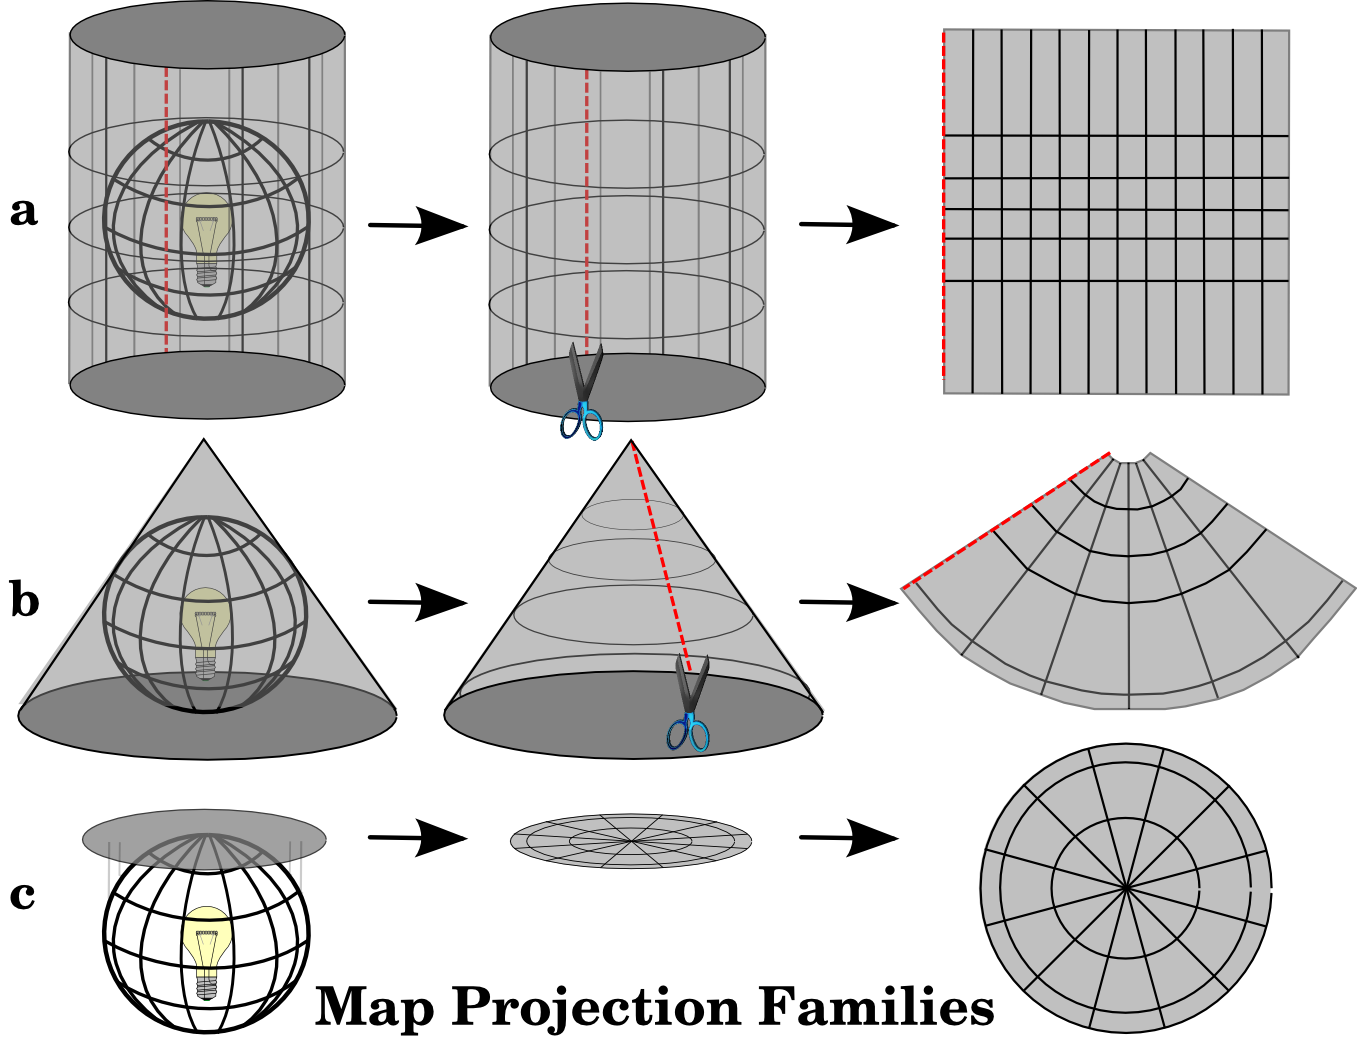
\includegraphics[clip=true, width=\textwidth]{projection-family}
\end{center}
\end{figure}

\subsection{Accuracy of map projections}

Map projections are never absolutely accurate representations of the
spherical earth. As a result of the map projection process, every map shows
\textbf{distortions of angular conformity, distance and area}. A map
projection may
combine several of these characteristics, or may be a compromise that
distorts all the properties of area, distance and angular conformity, within
some acceptable limit. Examples of compromise projections are the
\textbf{Winkel Tripel projection} and the \textbf{Robinson projection} (see
Figure \ref{fig:robinson}), which are often used for world maps. 

\begin{figure}[ht]
   \begin{center}
   \caption{The Robinson projection is a compromise where distortions of
area, angular conformity and distance are acceptable.}
\label{fig:robinson}\smallskip
   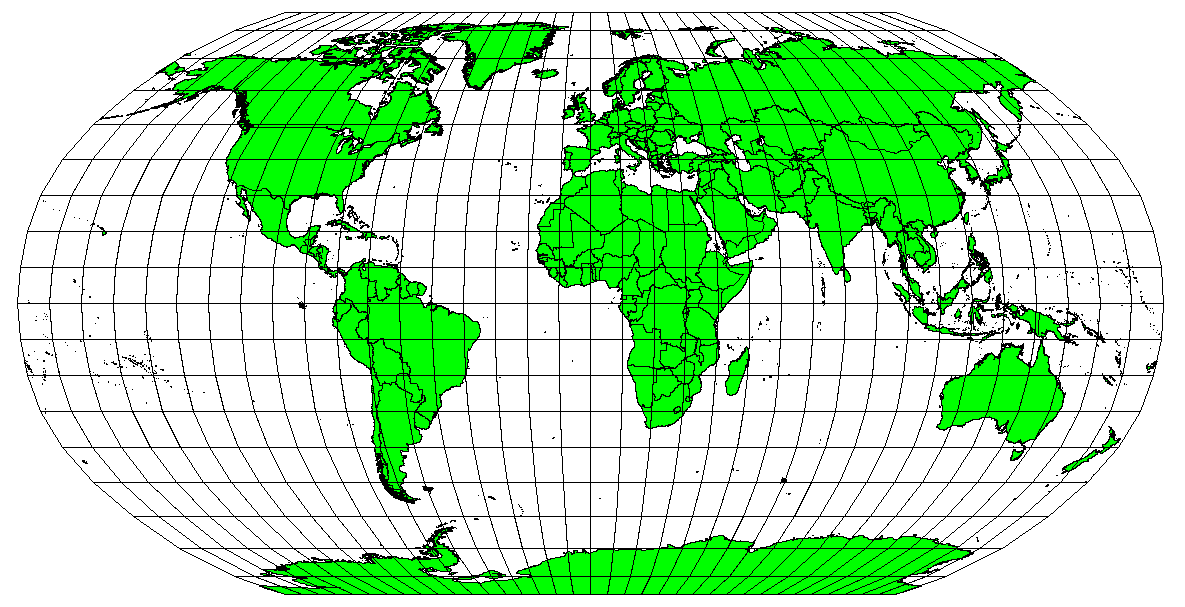
\includegraphics[clip=true, width=0.7\textwidth]{robinson-projection}
\end{center}
\end{figure}

It is usually impossible to preserve all characteristics at the same time in
a map projection. This means that when you want to carry out accurate
analytical operations, you need to use a map projection that provides the
best characteristics for your analyses. For example, if you need to measure
distances on your map, you should try to use a map projection for your data
that provides high accuracy for distances.

\subsection{Map projections with angular conformity}

When working with a globe, the main directions of the compass rose (North,
East, South and West) will always occur at 90 degrees to one another. In
other words, East will always occur at a 90 degree angle to North.
Maintaining correct \textbf{angular properties} can be preserved on a map
projection as well. A map projection that retains this property of angular
conformity is called a \textbf{conformal or orthomorphic projection}. 

\begin{figure}[ht]
   \begin{center}
   \caption{The Mercator projection, for example, is used where angular
relationships are important, but the relationship of areas are distorted.}
\label{fig:mercator}\smallskip
   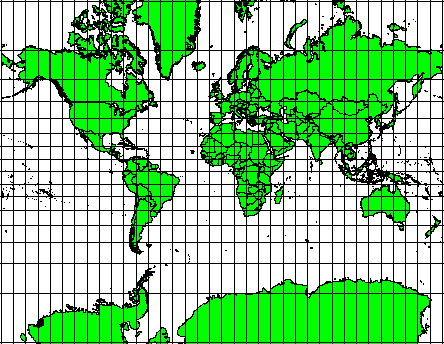
\includegraphics[clip=true, width=0.7\textwidth]{mercator-projection}
\end{center}
\end{figure}

These projections are used when the \textbf{preservation of angular
relationships} is
important. They are commonly used for navigational or meteorological tasks.
It is important to remember that maintaining true angles on a map is
difficult for large areas and should be attempted only for small portions of
the earth.  The conformal type of projection results in distortions of areas,
meaning that if area measurements are made on the map, they will be
incorrect. The larger the area the less accurate the area measurements will
be. Examples are the \textbf{Mercator projection} (as shown in Figure
ref{fig:mercator}) and the \textbf{Lambert Conformal Conic projection}. The
U.S. Geological Survey uses a conformal projection for many of its
topographic maps.

\subsection{Map projections with equal distance}

If your goal in projecting a map is to accurately measure distances, you
should select a projection that is designed to preserve distances well. Such
projections, called \textbf{equidistant projections}, require that the
\textbf{scale} of the map is \textbf{kept constant}. A map is equidistant
when it correctly represents
distances from the centre of the projection to any other place on the map.
\textbf{Equidistant projections} maintain accurate distances from the centre of the
projection or along given lines. These projections are used for radio and
seismic mapping, and for navigation. The \textbf{Plate Carree Equidistant
Cylindrical} (see Figure \ref{fig:platte}) and the \textbf{Equirectangular
projection} are two good examples of equidistant projections. The
\textbf{Azimuthal Equidistant projection} is
the projection used for the emblem of the United Nations (see Figure
\ref{fig:uno}).

\begin{figure}[ht]
   \begin{center}
   \caption{The United Nations Logo uses the Azimuthal Equidistant
projection.}
\label{fig:uno}\smallskip
   
\includegraphics[clip=true, width=0.3\textwidth]{unlogo}
\end{center}
\end{figure}

\begin{figure}[ht]
   \begin{center}
   \caption{The Plate Carree Equidistant Cylindrical projection, for example,
is used when accurate distance measurement is important.}
\label{fig:platte}\smallskip
   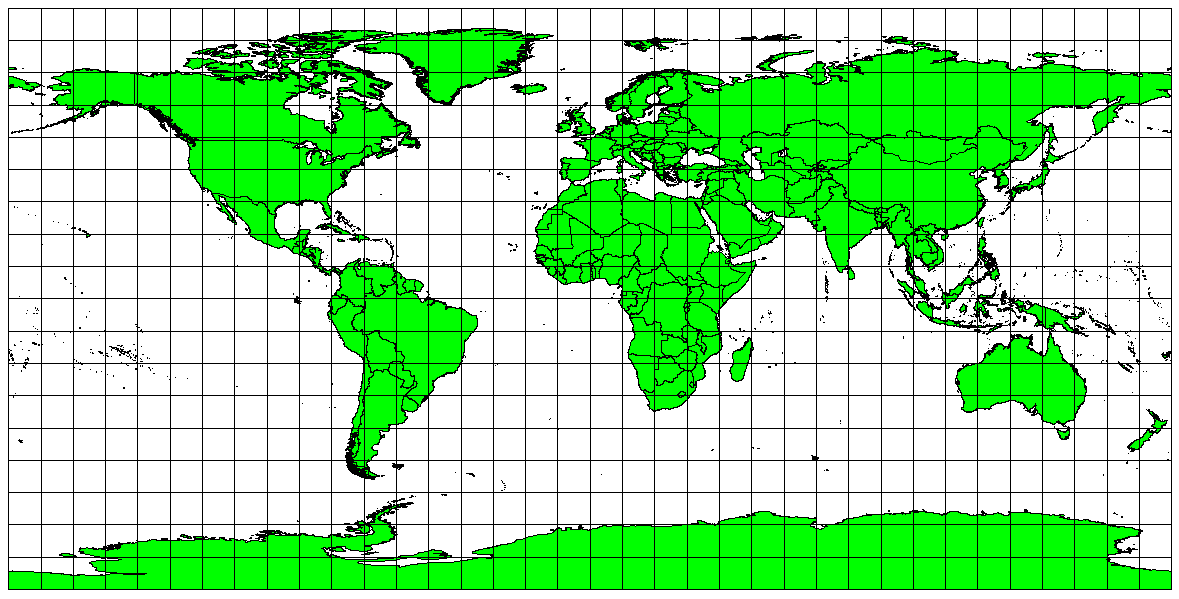
\includegraphics[clip=true, width=0.8\textwidth]{platte-carree-projection}
\end{center}
\end{figure}

\subsection{Projections with equal areas}

When a map portrays areas over the entire map, so that all mapped areas have
the same proportional relationship to the areas on the Earth that they
represent, the map is an \textbf{equal area map}. In practice, general reference and
educational maps most often require the use of \textbf{equal area
projections}. As the
name implies, these maps are best used when calculations of area are the
dominant calculations you will perform. If, for example, you are trying to
analyse a particular area in your town to find out whether it is large enough
for a new shopping mall, equal area projections are the best choice. On the
one hand, the larger the area you are analysing, the more precise your area
measures will be, if you use an equal area projection rather than another
type. On the other hand, an equal area projection results in
\textbf{distortions of angular conformity} when dealing with large areas.
Small areas will be far
less prone to having their angles distorted when you use an equal area
projection. \textbf{Alber's Equal Area, Lambert's Equal Area and Mollweide
Equal Area Cylindrical projections} (shown in Figure \ref{fig:mollweide}) are
types of equal area projections that are often encountered in GIS work.

Keep in mind that map projection is a very complex topic. There are hundreds
of different projections available world wide each trying to portray a
certain portion of the earth's surface as faithfully as possible on a flat
piece of paper. In reality, the choice of which projection to use, will often
be made for you. Most countries have commonly used projections and when data
is exchanged people will follow the \textbf{national trend}.

\begin{figure}[ht]
   \begin{center}
   \caption{The Mollweide Equal Area Cylindrical projection, for example,
ensures that all mapped areas have the same proportional relationship to the
areas on the Earth.}
\label{fig:mollweide}\smallskip
   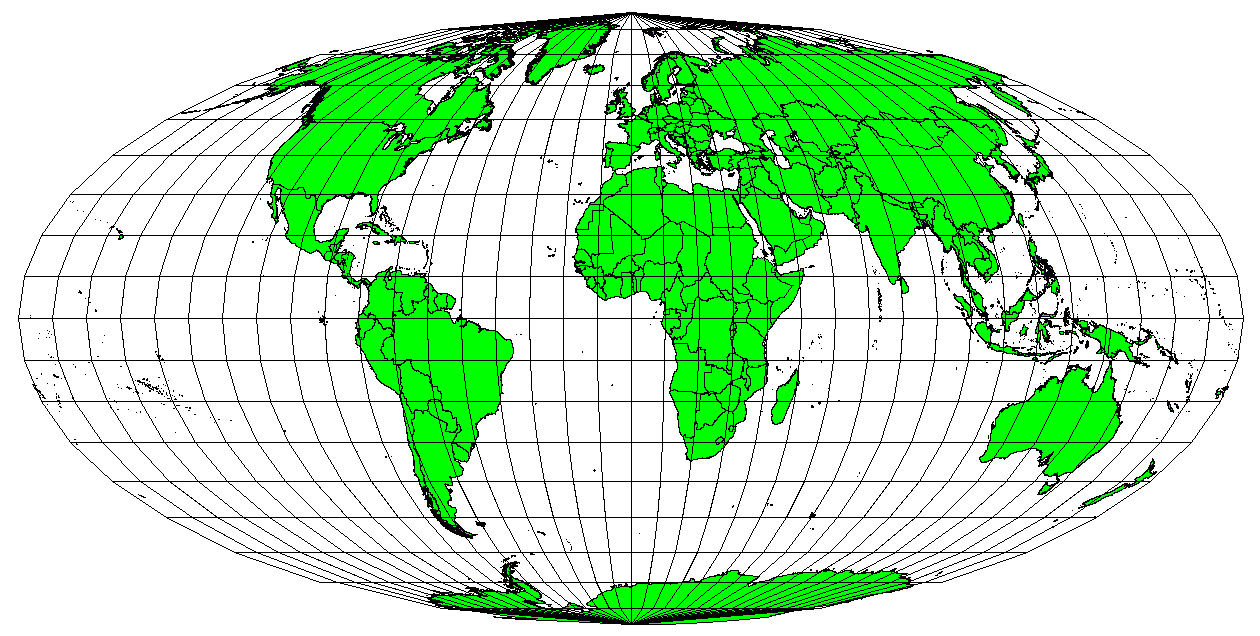
\includegraphics[clip=true, width=0.8\textwidth]{mollweide_equal_area_projection}
\end{center}
\end{figure}

\subsection{Coordinate Reference System (CRS) in detail}

With the help of coordinate reference systems (CRS) every place on the earth
can be specified by a set of three numbers, called coordinates. In general
CRS can be divided into \textbf{projected coordinate reference systems} (also
called Cartesian or rectangular coordinate reference systems) and
\textbf{geographic coordinate reference systems}. 

\subsection{Geographic Coordinate Systems}

The use of Geographic Coordinate Reference Systems is very common. They use
degrees of latitude and longitude and sometimes also a height value to
describe a location on the earth's surface. The most popular is called
\textbf{WGS 84}.

\textbf{Lines of latitude} run parallel to the equator and divide the earth into 180
equally spaced sections from North to South (or South to North). The
reference line for latitude is the equator and each \textbf{hemisphere} is
divided
into ninety sections, each representing one degree of latitude. In the
northern hemisphere, degrees of latitude are measured from zero at the
equator to ninety at the north pole. In the southern hemisphere, degrees of
latitude are measured from zero at the equator to ninety degrees at the south
pole. To simplify the digitisation of maps, degrees of latitude in the
southern hemisphere are often assigned negative values (0 to -90$^\circ$). Wherever
you are on the earth's surface, the distance between the lines of latitude is
the same (60 nautical miles). See Figure \ref{fig:latlon} for a pictorial view.

\begin{figure}[ht]
   \begin{center}
   \caption{Geographic coordinate system with lines of latitude parallel to
the equator and lines of longitude with the prime meridian through Greenwich.}
\label{fig:latlon}\smallskip
   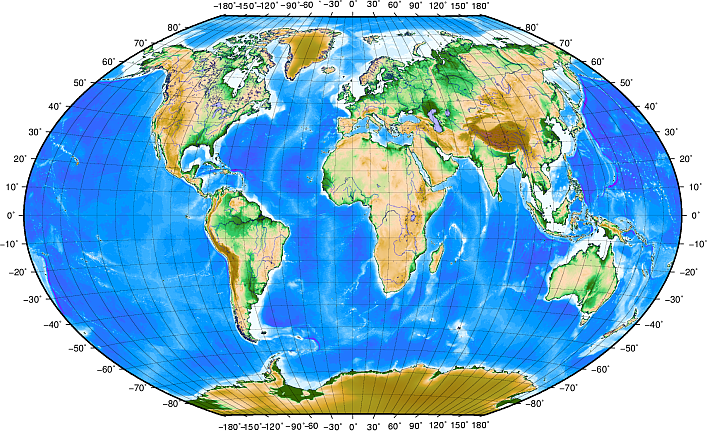
\includegraphics[clip=true, width=0.8\textwidth]{latlon}
\end{center}
\end{figure}

\textbf{Lines of longitude}, on the other hand, do not stand up so well to the
standard of uniformity. Lines of longitude run perpendicular to the equator
and converge at the poles. The reference line for longitude (the prime
meridian) runs from the North pole to the South pole through Greenwich,
England. Subsequent lines of longitude are measured from zero to 180 degrees
East or West of the prime meridian. Note that values West of the prime
meridian are assigned negative values for use in digital mapping
applications. See Figure \ref{fig:latlon} for a pictorial view.

At the equator, and only at the equator, the distance represented by one line
of longitude is equal to the distance represented by one degree of latitude.
As you move towards the poles, the distance between lines of longitude
becomes progressively less, until, at the exact location of the pole, all
360$^\circ$ of longitude are represented by a single point that you could put your
finger on (you probably would want to wear gloves though). Using the
geographic coordinate system, we have a grid of lines dividing the earth into
squares that cover approximately 12363.365 square kilometres at the equator -
a good start, but not very useful for determining the location of anything
within that square.

To be truly useful, a map grid must be divided into small enough sections so
that they can be used to describe (with an acceptable level of accuracy) the
location of a point on the map. To accomplish this, degrees are divided into
\textbf{minutes (')} and \textbf{seconds (")}. There are sixty minutes in a
degree, and sixty
seconds in a minute (3600 seconds in a degree). So, at the equator, one
second of latitude or longitude = 30.87624 meters.

\subsection{Projected coordinate reference systems}

A two-dimensional coordinate reference system is commonly defined by two
axes. At right angles to each other, they form a so called \textbf{XY}-plane
(see Figure \ref{fig:crsaxes} on the left side). The horizontal axis is normally
labelled \textbf{X}, and the vertical axis is normally labelled \textbf{Y}.
In a three-dimensional coordinate reference system, another axis, normally
labelled \textbf{Z}, is added. It
is also at right angles to the \textbf{X} and \textbf{Y} axes. The Z axis
provides the third
dimension of space (see Figure \ref{fig:crsaxes} on the right side).  Every
point that
is expressed in spherical coordinates can be expressed as an \textbf{X Y Z}
coordinate. 

\begin{figure}[ht]
   \begin{center}
   \caption{Two and three dimensional coordinate reference systems}
\label{fig:crsaxes}\smallskip
   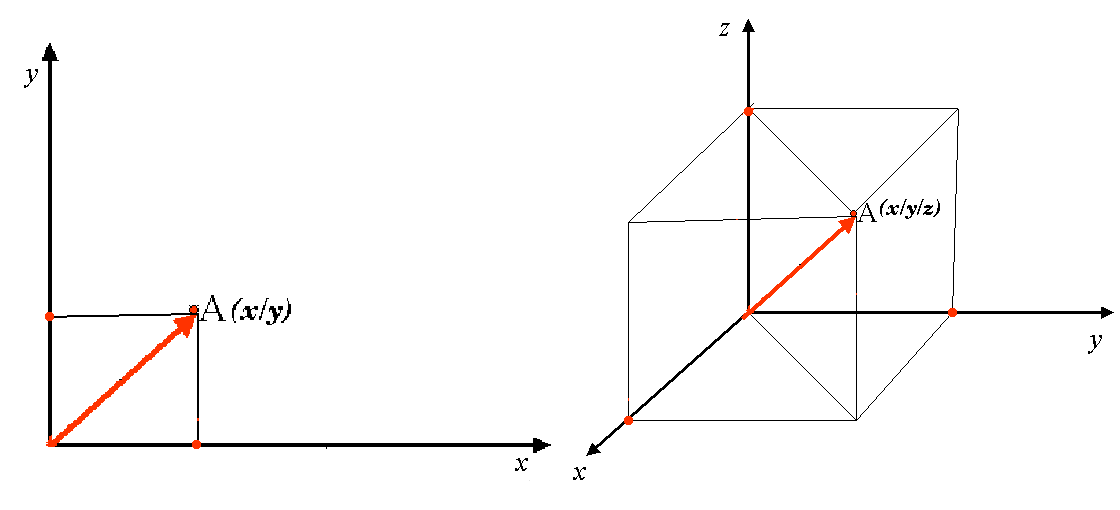
\includegraphics[clip=true, width=\textwidth]{cartesian-system}
\end{center}
\end{figure}

A projected coordinate reference system in the southern hemisphere (south of
the equator) normally has its origin on the equator at a specific
\textbf{Longitude}.
This means that the Y-values increase southwards and the X-values increase to
the West. In the northern hemisphere (north of the equator) the origin is
also the equator at a specific \textbf{Longitude}. However, now the Y-values
increase
northwards and the X-values increase to the East. In the following section,
we describe a projected coordinate reference system, called \textbf{Universal
Transverse Mercator} (UTM) often used for South Africa. 

\subsubsection{Universal Transverse Mercator (UTM) CRS in detail}

The Universal Transverse Mercator (UTM) coordinate reference system has its
origin on the \textbf{equator} at a specific \textbf{Longitude}. Now the
Y-values increase
Southwards and the X-values increase to the West. The UTM CRS is a global map
projection. This means, it is generally used all over the world. But as
already described in the section 'accuracy of map projections' above, the
larger the area (for example South Africa) the more distortion of angular
conformity, distance and area occur. To avoid too much distortion, the world
is divided into \textbf{60 equal zones} that are all \textbf{6 degrees} wide
in longitude from
East to West. The \textbf{UTM zones} are numbered \textbf{1 to 60}, starting
at the \textbf{international date line} (\textbf{zone 1} at 180 degrees West
longitude) and progressing East back to the \textbf{international date line}
(\textbf{zone 60} at 180 degrees East longitude) as shown in Figure
\ref{fig:utmzones}.

\begin{figure}[ht]
   \begin{center}
   \caption{The Universal Transverse Mercator zones. For South Africa UTM
zones 33S, 34S, 35S, and 36S are used.}
\label{fig:utmzones}\smallskip
   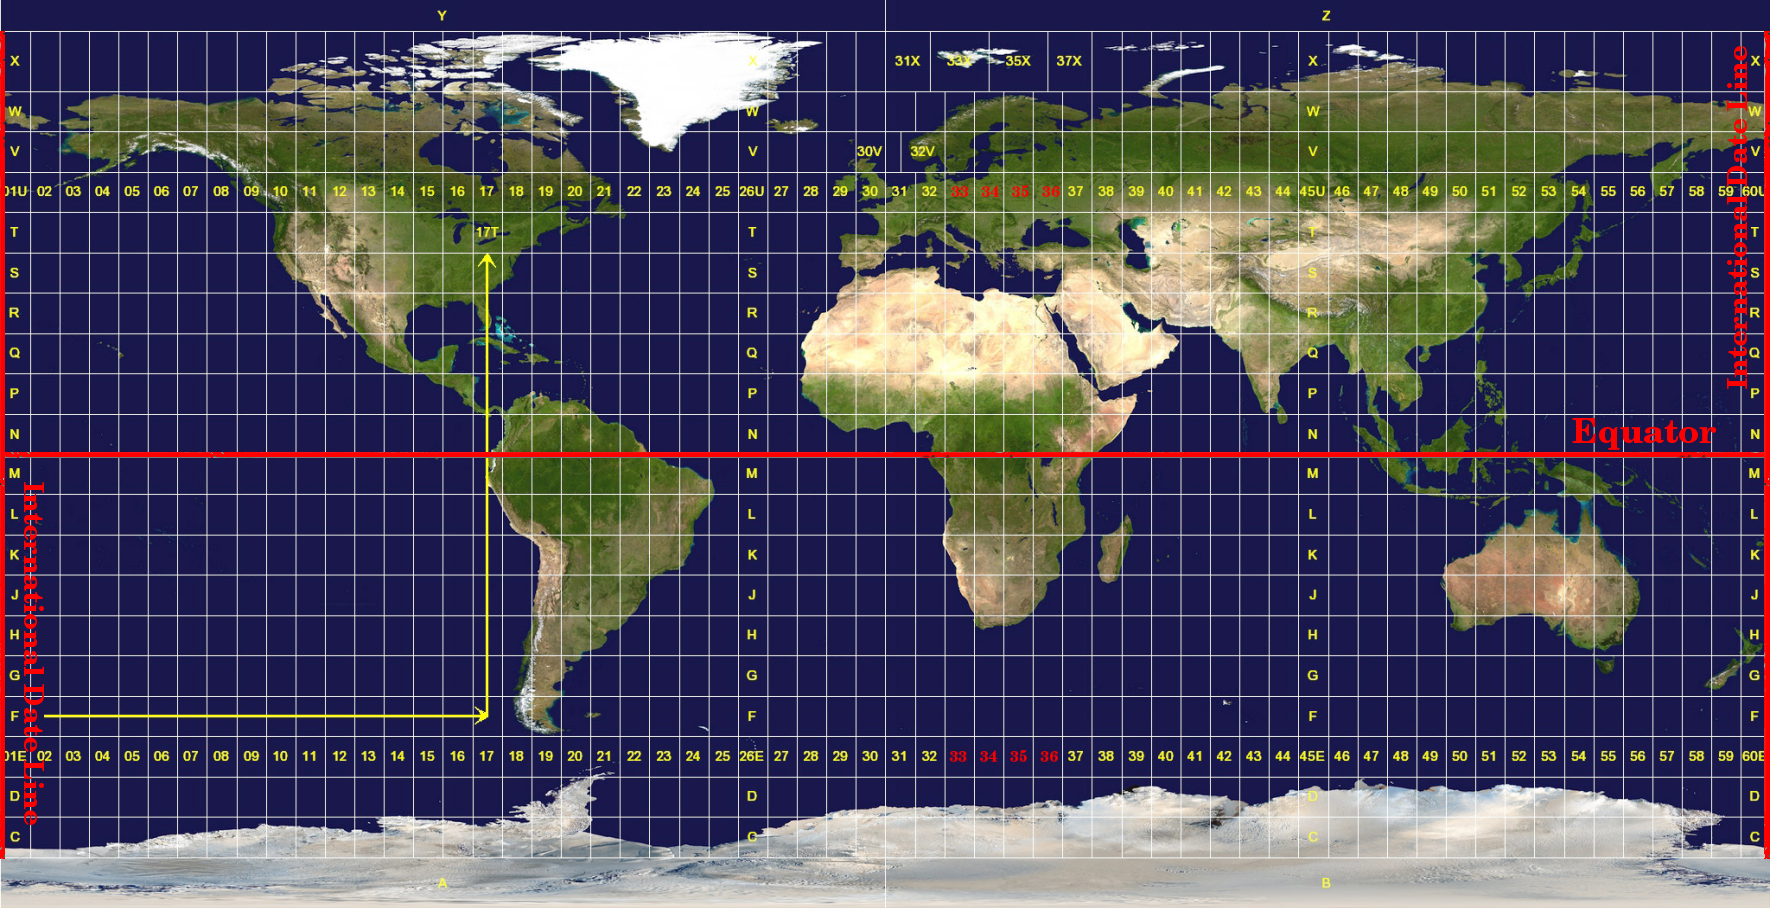
\includegraphics[clip=true, width=\textwidth]{utmzones}
\end{center}
\end{figure}

As you can see in Figure \ref{fig:utmzones} and Figure \ref{fig:zautmzones},
South Africa is covered by four \textbf{UTM zones} to minimize distortion.
The \textbf{zones} are called \textbf{UTM 33S, UTM 34S, UTM 35S} and
\textbf{UTM 36S}. The \textbf{S} after the zone means that
the UTM zones are located \textbf{south of the equator}.

\begin{figure}[ht]
   \begin{center}
   \caption{UTM zones 33S, 34S, 35S, and 36S with their central longitudes
(meridians) used to project South Africa with high accuracy. The red cross
shows an Area of Interest (AOI).}
\label{fig:zautmzones}\smallskip
   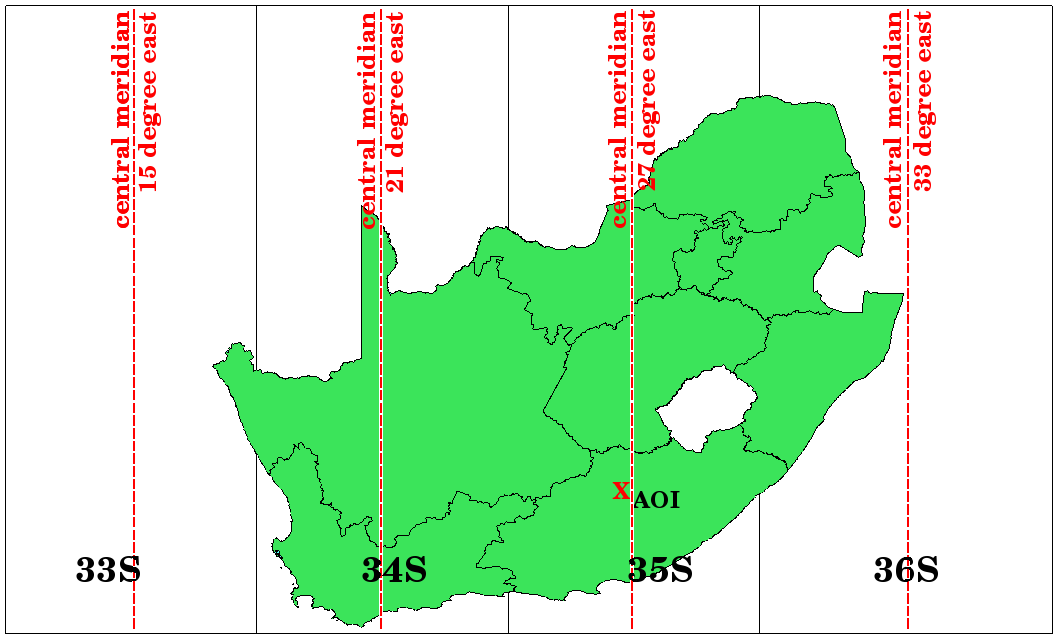
\includegraphics[clip=true, width=0.8\textwidth]{za_utmzones}
\end{center}
\end{figure}

Say, for example, that we want to define a two-dimensional coordinate within
the \textbf{Area of Interest (AOI)} marked with a red cross in Figure
\ref{fig:zautmzones}.
You can see, that the area is located within the \textbf{UTM zone 35S}. This
means, to
minimize distortion and to get accurate analysis results, we should use
\textbf{UTM zone 35S} as the coordinate reference system. 

The position of a coordinate in UTM south of the equator must be indicated
with the \textbf{zone number} (35) and with its \textbf{northing (y) value}
and \textbf{easting (x) value} in  meters. The \textbf{northing value} is the
distance of the position from the \textbf{equator} in meters. The
\textbf{easting value} is the distance from the \textbf{central
meridian} (longitude) of the used UTM zone. For UTM zone 35S it is \textbf{27
degrees East} as shown in Figure \ref{fig:zautmzones}. Furthermore, because
we are south of
the equator and negative values are not allowed in the UTM coordinate
reference system, we have to add a so called \textbf{false northing value} of
10,000,000m to the northing (y) value and a false easting value of 500,000m
to the easting (x) value.  

This sounds difficult, so, we will do an example that shows you how to find
the correct \textbf{UTM 35S} coordinate for the \textbf{Area of Interest}. 

\minisec{The northing (y) value}

The place we are looking for is 3,550,000 meters south of the equator, so the
northing (y) value gets a \textbf{negative sign} and is -3,550,000m.
According to the
UTM definitions we have to add a \textbf{false northing value} of
10,000,000m. This
means the northing (y) value of our coordinate is 6,450,000m (-3,550,000m +
10,000,000m).

\minisec{The easting (x) value}

First we have to find the \textbf{central meridian} (longitude) for the
\textbf{UTM zone 35S}.
As we can see in ***71*** it is \textbf{27 degrees East}. The place we are
looking for
is \textbf{85,000 meters West} from the central meridian. Just like the northing
value, the easting (x) value gets a negative sign, giving a result of
\textbf{-85,000m}. According to the UTM definitions we have to add a
\textbf{false easting value} of 500,000m. This means the easting (x) value of
our coordinate is
415,000m (-85,000m + 500,000m). Finally, we have to add the \textbf{zone
number} to the easting value to get the correct value.

As a result, the coordinate for our \textbf{Point of Interest}, projected in
\textbf{UTM zone 35S} would be written as: \textbf{35 415,000mE /
6,450,000mN}. In some GIS, when the
correct UTM zone 35S is defined and the units are set to meters within the
system, the coordinate could also simply appear as \textbf{415,000 6,450,000}.

\subsection{On-The-Fly Projection}

As you can probably imagine, there might be a situation where the data you
want to use in a GIS are projected in different coordinate reference systems.
For example, you might get a vector layer showing the boundaries of South
Africa projected in UTM 35S and another vector layer with point information
about rainfall provided in the geographic coordinate system WGS 84. In GIS
these  two vector layers are placed in totally different areas of the map
window, because they have different projections.

To solve this problem, many GIS include a functionality called
\textbf{On-the-fly} projection. It means, that you can \textbf{define} a
certain projection when you start
the GIS and all layers that you then load, no matter what coordinate
reference system they have, will be automatically displayed in the projection
you defined. This functionality allows you to overlay layers within the map
window of your GIS, even though they may be in \textbf{different} reference
systems.

\subsection{Common problems / things to be aware of}

The topic \textbf{map projection} is very complex and even professionals who have
studied geography, geodetics or any other GIS related science, often have
problems with the correct definition of map projections and coordinate
reference systems. Usually when you work with GIS, you already have projected
data to start with. In most cases these data will be projected in a certain
CRS, so you don't have to create a new CRS or even re project the data from
one CRS to another. That said, it is always useful to have an idea about what
map projection and CRS means. 

\subsection{What have we learned?}

Let's wrap up what we covered in this worksheet:

\begin{itemize}
\item \textbf{Map projections} portray the surface of the earth on a two-dimensional, flat
piece of paper or computer screen. 
\item There are global map projections, but most map projections are created and
\textbf{optimized to project smaller areas} of the earth's surface.
\item Map projections are never absolutely accurate representations of the
spherical earth. They show \textbf{distortions of angular conformity, distance and
area}. It is impossible to preserve all these characteristics at the same time
in a map projection.
\item \textbf{A Coordinate reference system} (CRS) defines, with the help of
coordinates,
how the two-dimensional, projected map is related to real locations on the
earth.
\item There are two different types of coordinate reference systems:
\textbf{Geographic Coordinate Systems} and \textbf{Projected Coordinate
Systems}.
\item \textbf{On the Fly projection} is a functionality in GIS that allows us
to overlay
layers, even if they are projected in different coordinate reference systems.
\end{itemize}

\subsection{Now you try!}

Here are some ideas for you to try with your learners:

\begin{itemize}
\item Start QGIS and load two layers of the same area but with different
projections and let your pupils find the coordinates of several places on the
two layers. You can show them that it is not possible to overlay the two
layers. Then define the coordinate reference system as Geographic/ WGS 84
inside the Project Properties Dialog and activate the check box 'enable
On-the-fly CRS transformation'. Load the two layers of the same area again
and let your pupils see how On-the-fly projection works.
\item You can open the Project Properties Dialog in QGIS and show your pupils the
many different Coordinate Reference Systems so they get an idea of the
complexity of this topic. With 'On-the-fly CRS transformation' enabled you
can select different CRS to display the same layer in different projections.
\end{itemize}

\subsection{Something to think about}

If you don't have a computer available, you can show your pupils the
principles of the three map projection families. Get a globe and paper and
demonstrate how cylindrical, conical and planar projections work in general.
With the help of a transparency sheet you can draw a two-dimensional
coordinate reference system showing X axes and Y axes. Then, let your pupils
define coordinates (x and y values) for different places. 

\subsection{Further reading}

\textbf{Books}:

\begin{itemize}
\item Chang, Kang-Tsung (2006): Introduction to Geographic Information Systems. 3rd
Edition.  McGraw Hill. (ISBN 0070658986)
\item DeMers, Michael N. (2005): Fundamentals of Geographic Information Systems.
3rd Edition. Wiley. (ISBN 9814126195)
\item Galati, Stephen R. (2006): Geographic Information Systems Demystified. Artech
House Inc. (ISBN 158053533X)
\end{itemize}

\textbf{Websites}: 

\url{http://www.colorado.edu/geography/gcraft/notes/mapproj/mapproj_f.html}
\\
\url{http://geology.isu.edu/geostac/Field_Exercise/topomaps/index.htm}

The QGIS User Guide also has more detailed information on working with map
projections in QGIS.

\subsection{What's next?}

In the section that follows we will take a closer look at \textbf{Map Production}.


